\documentclass[12pt]{report}
\usepackage{amssymb}
\usepackage{amsmath}

\usepackage{multicol}
\usepackage{graphicx}
\usepackage{subfigure}
\usepackage{verbatim}

%\usepackage{adjustbox}

\usepackage[letterpaper,left=1cm,right=2cm, top=1.5cm,
bottom=1.5cm,head=0cm,foot=1cm]{geometry}

\parindent=0in


\newcommand{\m}{\mbox{m }}
\newcommand{\kg}{\mbox{kg}}
\newcommand{\s}{\mbox{s}}
\newcommand{\ke}{\mbox{\small KE}}
\newcommand{\pe}{\mbox{\small PE}}
\newcommand{\un}{\mbox{ u}}


\newcommand{ \probDir}[1]{{ \bf\small #1 \mbox{  }}}

\newcommand{ \breakList}{\setcounter{saveenum}{\value{enumi}} \end{enumerate}}
\newcommand{ \contList}{\begin{enumerate} \setcounter{enumi}{\value{saveenum}}}

\newcounter{saveenum}

\def \wspace{5cm}

%%%%%%%%%%%%%%%%%%%%%%%%%%%%%%%%%%%%%%%%%
\begin{document}

{\bf{Honors Physics} \hfill Notepage: Inclined Plane \hfill {Mr. Kelley}} \\ \\
%%%%%%%%%%

\hfill 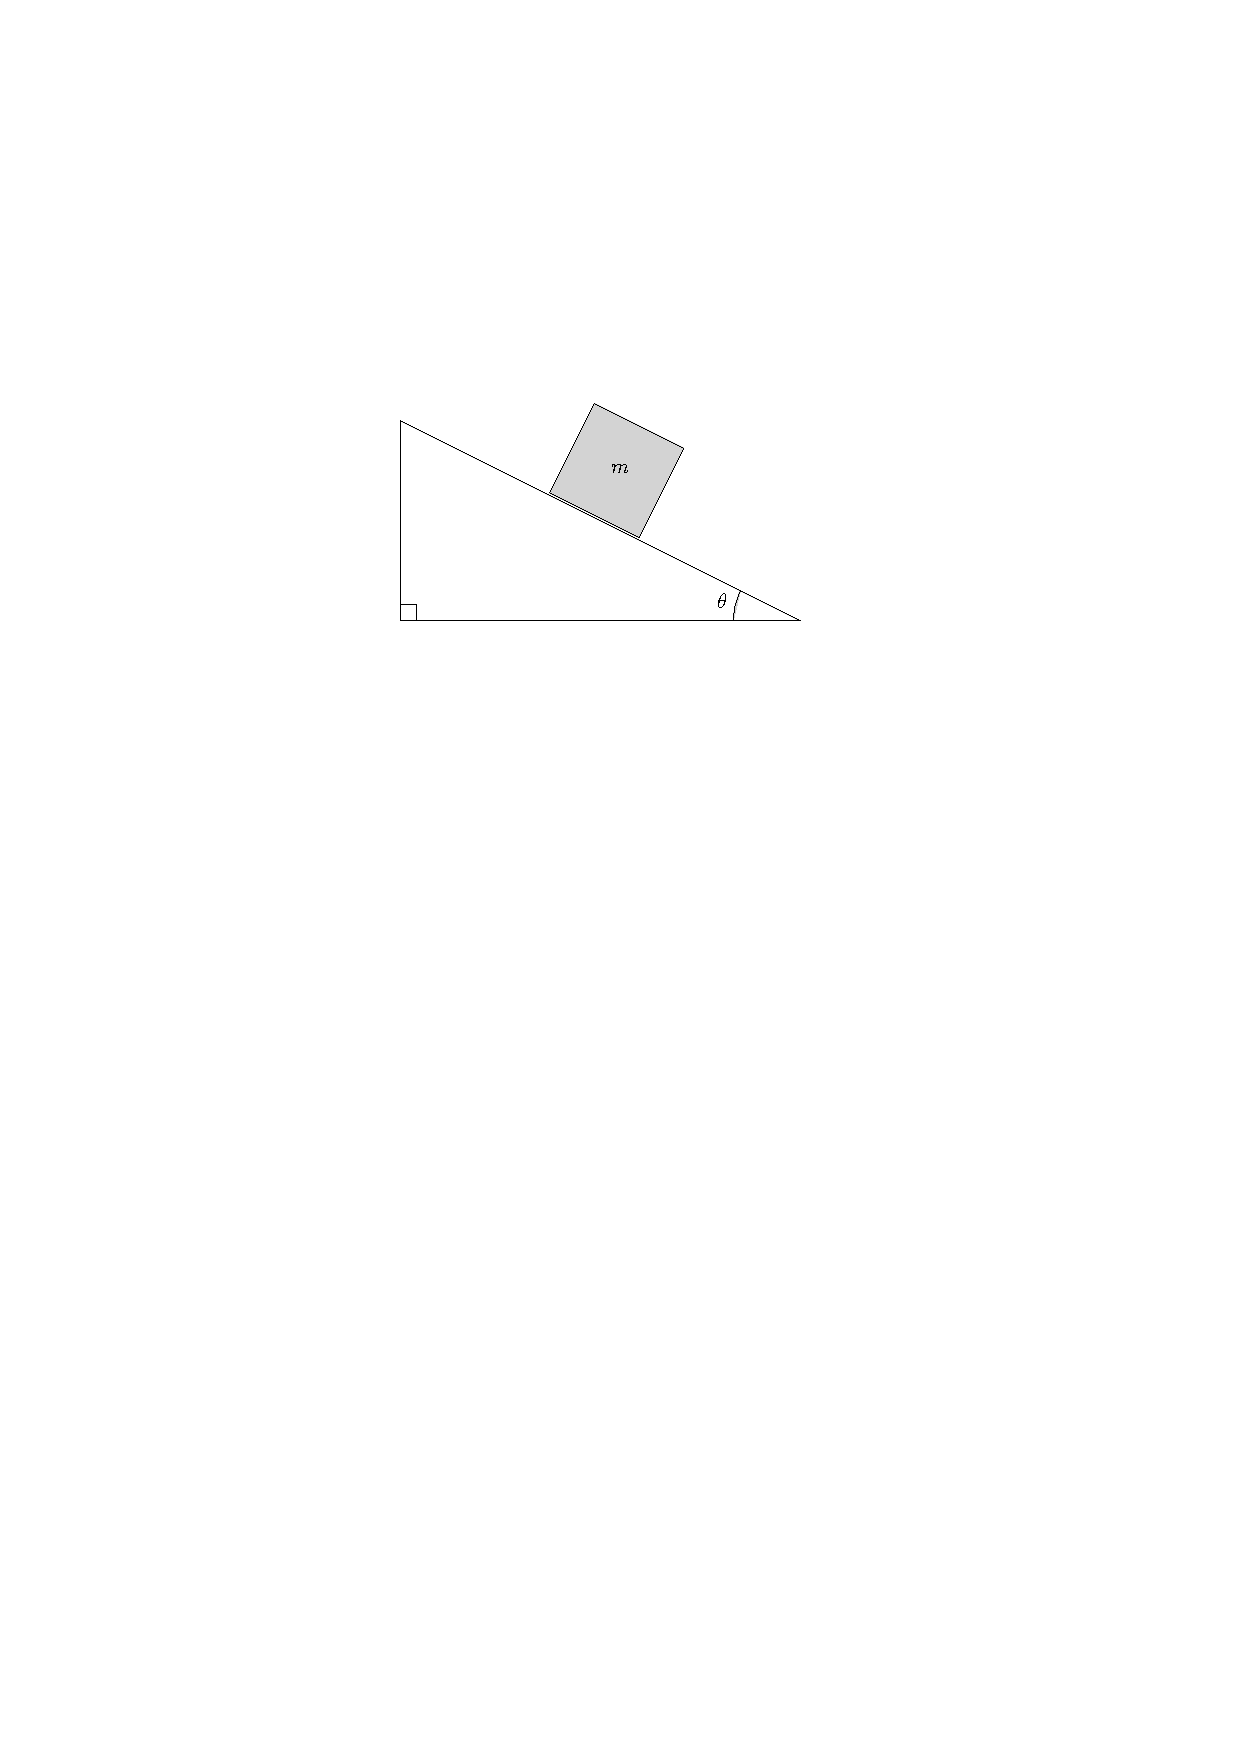
\includegraphics[scale = .75]{inclinedPlane_1} \hfill \mbox{}

\vspace{.5cm}

\hfill \parbox{12cm}{Now consider a mass on a surface that is \emph{not} horizontal.  All of the same concepts and equations apply.  The key to understanding the difference is understanding the normal force.  Remember $F_\bot$ is always perpendicular to the \emph{surface}.  This Notepage gives step-by-step instructions for drawing a triangle to understand the forces.} \hspace{4cm}

\vspace{.5cm}

\hfill \parbox{6cm}{The first force that we know about for sure is the force of gravity acting on the mass.  $F_g = mg$} \hfill \parbox{6cm}{We also know that the normal force must be perpendicular to the surface.} \hfill \mbox{}

\vspace{.75cm}

\hfill 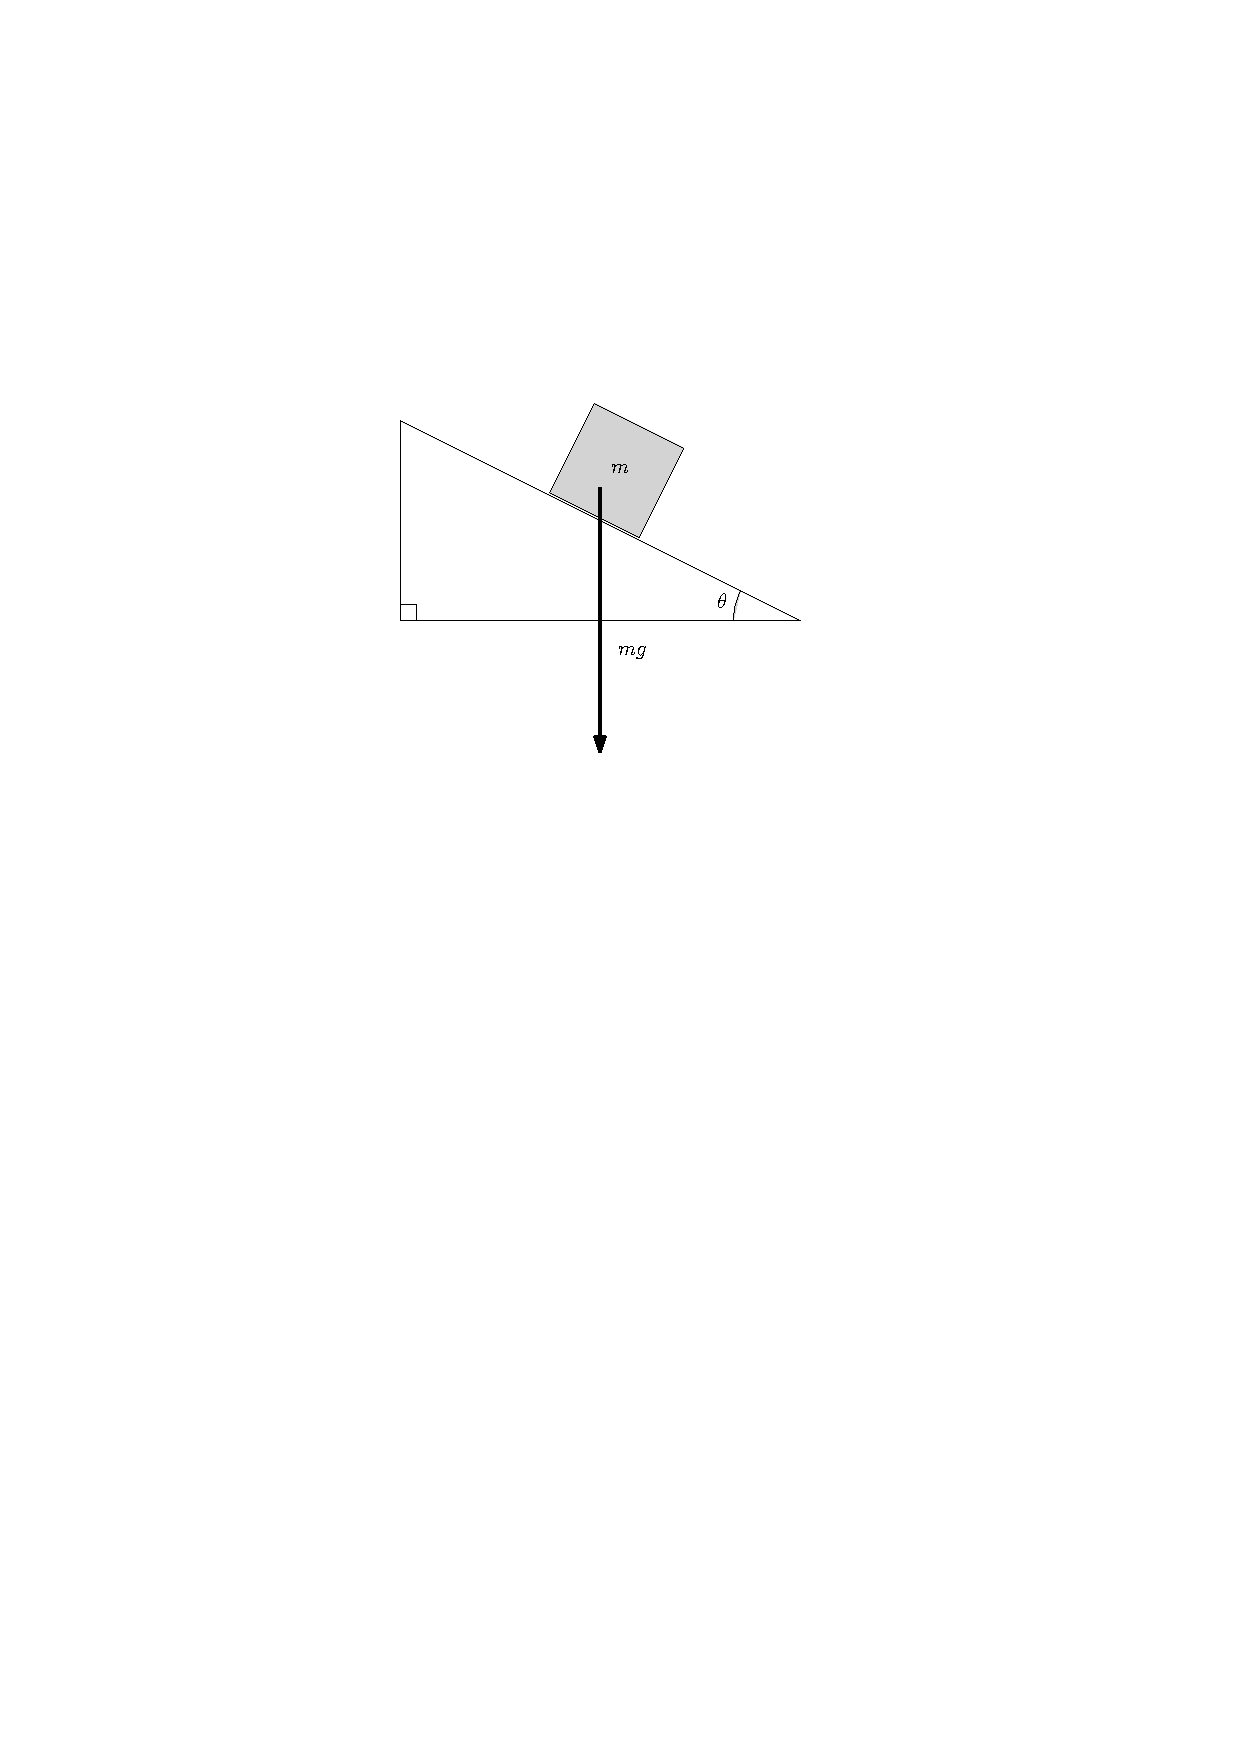
\includegraphics[scale = .75] {inclinedPlane_2} \hfill 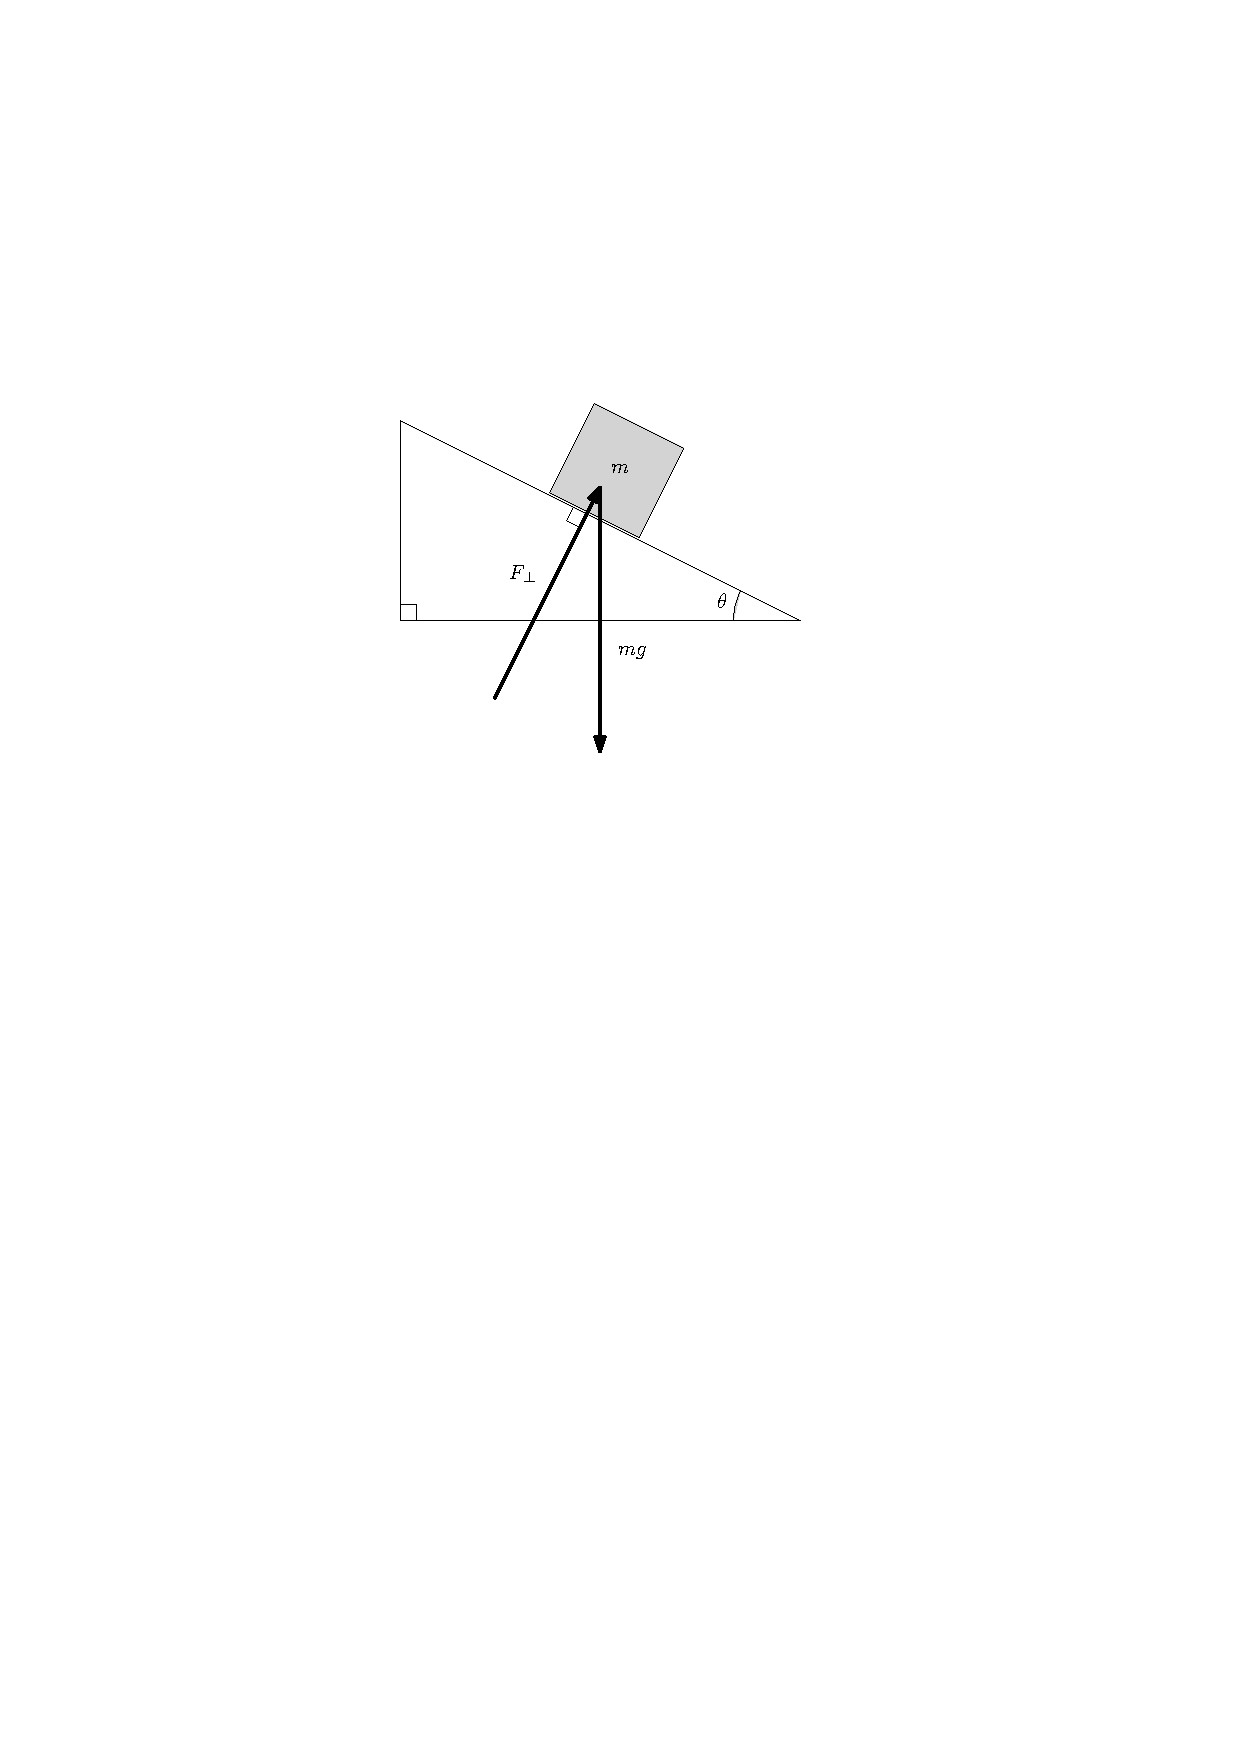
\includegraphics[scale = .75] {inclinedPlane_3} \hfill \mbox{}
\vspace{.75cm}

\hfill \parbox{14cm}{From here we use similar triangles to finish the force vectors.  Notice that $F_\|$ is parallel to the surface and $F_\bot$ is perpendicular.  $F_\|$ is the force "going down" the inclined plane.  If there is friction, it is in the opposite direction of $F_\|$.  The most common mistake in drawing this triangle is included below.  Notice that in the correct triangle, the right angles are closer together.} \hspace{3cm}

\hfill 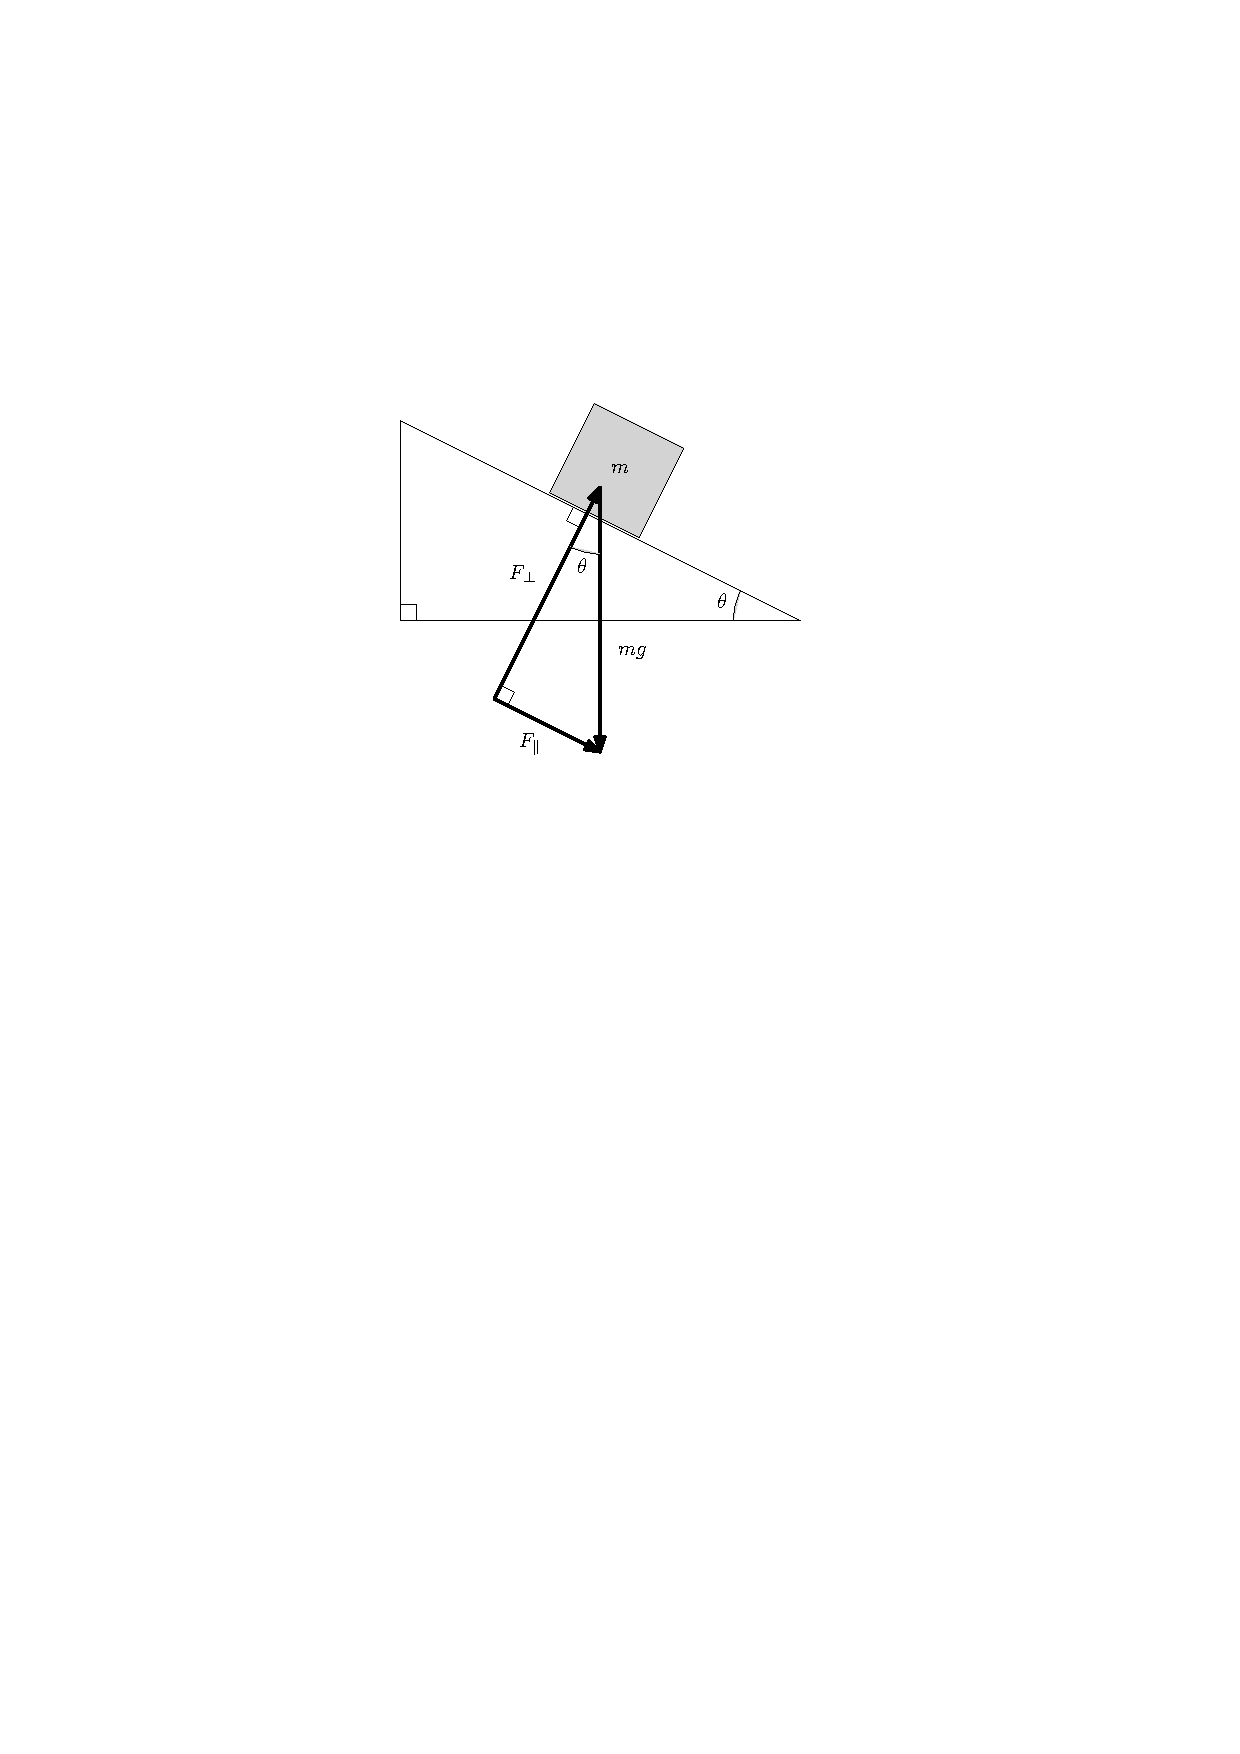
\includegraphics[scale = .95] {inclinedPlane} \hfill 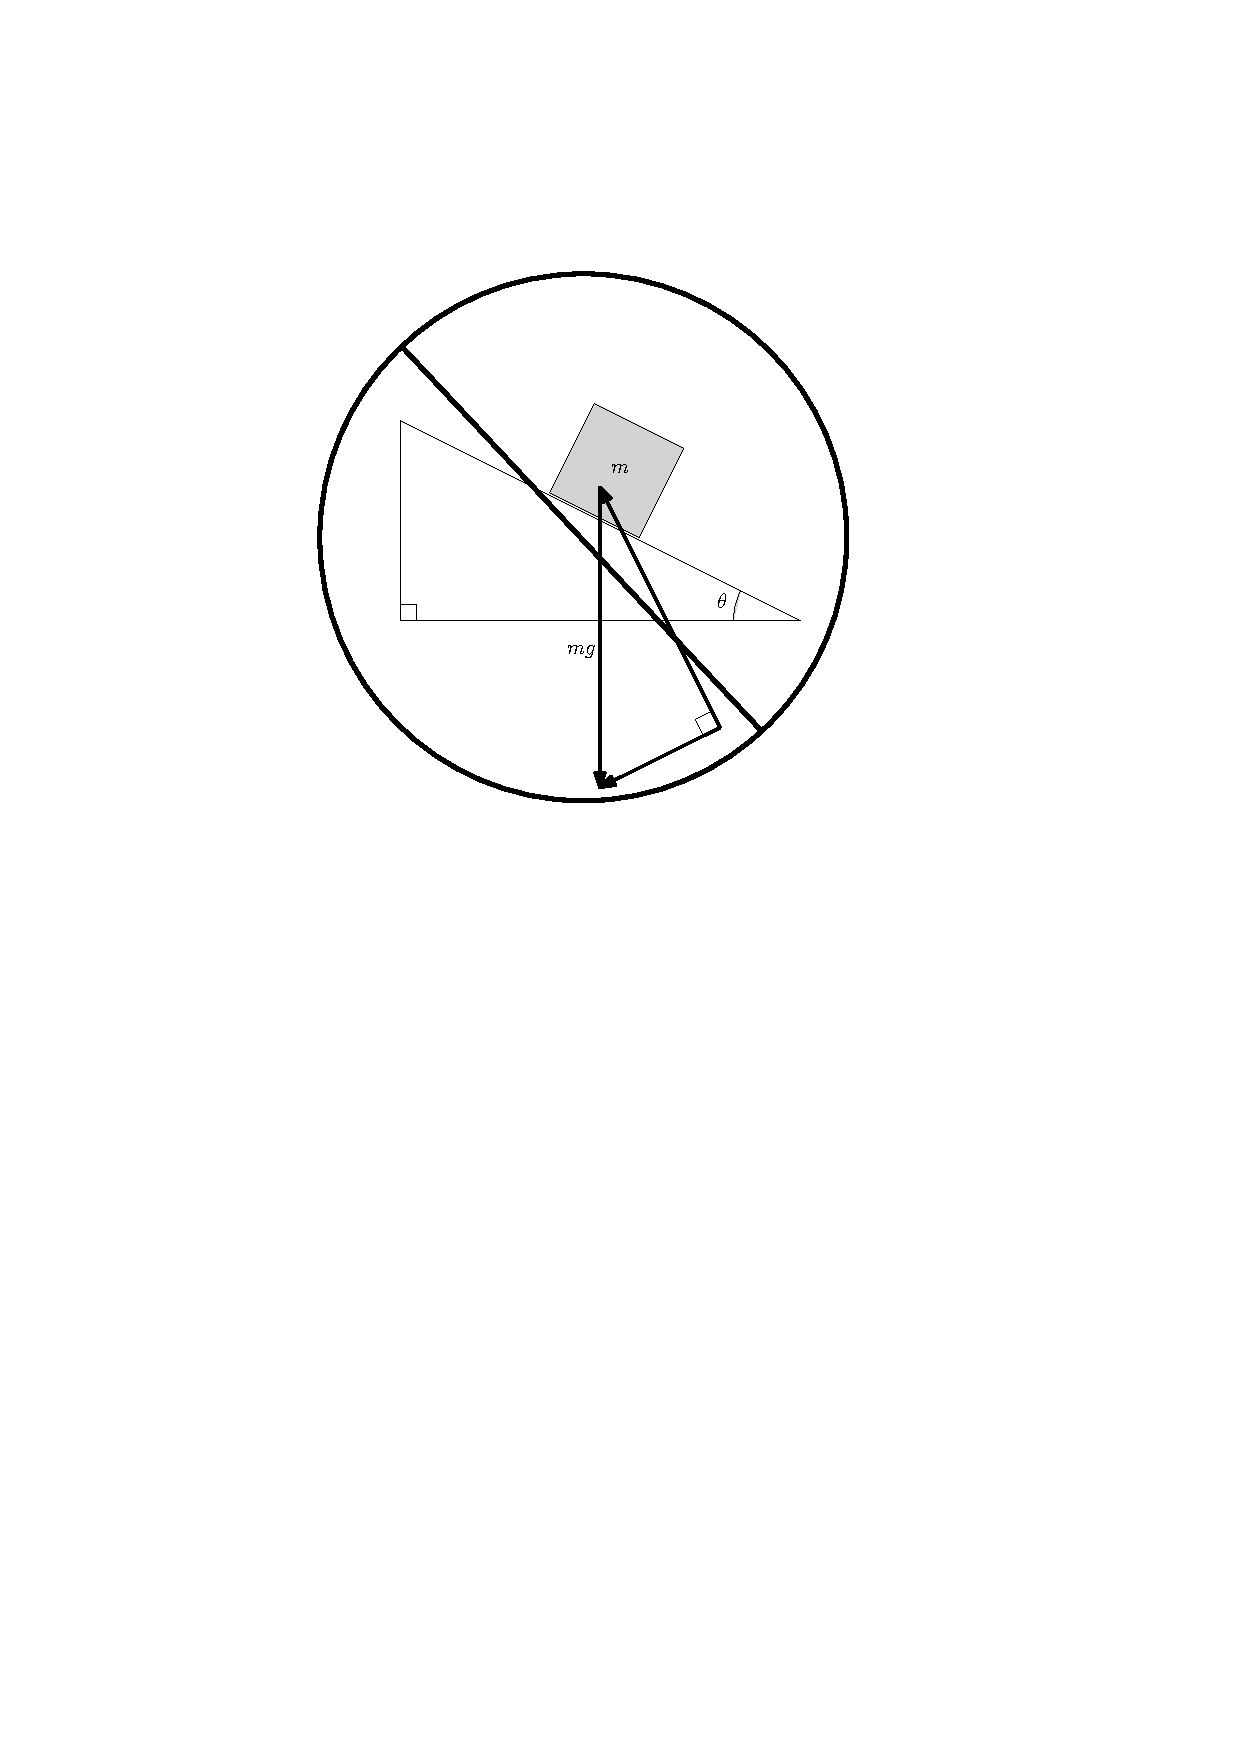
\includegraphics[scale = .75] {inclinedPlane_wrong} \hfill \mbox{}

\end{document}